\documentclass{standalone}
\usepackage{tikz}
\begin{document}
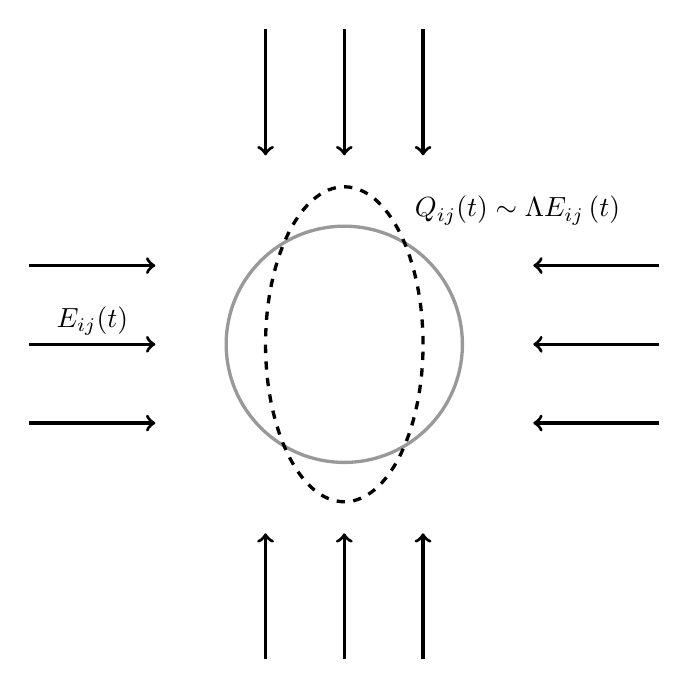
\begin{tikzpicture}
    \filldraw[color=black, fill=white,      opacity=0.4, very thick        ] (0,0) circle (1.5);
    \filldraw[color=black, fill=white, fill opacity=0,   very thick, dashed] (0,0) ellipse (1 and 2);
    \draw[very thick, ->] (-4, 1) -- (-2.4, 1);
    \draw[very thick, ->] (-4, 0) -- (-2.4, 0);
    \draw[very thick, ->] (-4,-1) -- (-2.4,-1);
    \draw[very thick, ->] (+4, 1) -- (+2.4, 1);
    \draw[very thick, ->] (+4, 0) -- (+2.4, 0);
    \draw[very thick, ->] (+4,-1) -- (+2.4,-1);
    \draw[very thick, ->] (+1,+4) -- (+1,+2.4);
    \draw[very thick, ->] ( 0,+4) -- ( 0,+2.4);
    \draw[very thick, ->] (-1,+4) -- (-1,+2.4);
    \draw[very thick, ->] (+1,-4) -- (+1,-2.4);
    \draw[very thick, ->] ( 0,-4) -- ( 0,-2.4);
    \draw[very thick, ->] (-1,-4) -- (-1,-2.4);
    \node[] at (-3.2,0.3) {$E_{ij}(t)$} ;
    \node[] at (2.2,1.7) {$Q_{ij}(t)\sim \Lambda E_{ij}\left(t\right)$} ;
\end{tikzpicture}
\end{document}
